\documentclass[12pt,a4paper]{article}
\usepackage{amsmath,amsfonts,amssymb}
\usepackage{fullpage}
\usepackage[utf8]{inputenc} 
\usepackage[T1]{fontenc}
\usepackage[french]{babel}
\usepackage{graphicx}
\usepackage{versions}
\usepackage{setspace}
\usepackage{pdfpages}
\usepackage{ulem}
\usepackage{csquotes}% package pour gérer les guillemets (requis pour biblatex)
\usepackage{hyperref}
\usepackage[left=1.5cm,right=2cm,top=1.5cm,bottom=2cm]{geometry}
\usepackage{xr-hyper} 


\usepackage[usenames,dvipsnames]{xcolor}
\definecolor{nameColor}{HTML}{59153A}

\begin{document}\


\begin{figure}\
	\flushright
		
\includegraphics[scale=0.2]{ups.png}
\end{figure}

\renewcommand\fbox{\fcolorbox{nameColor}{white}}
\fboxrule 2pt \fbox{
\parbox{15cm}{

\setlength{\parskip}{.10cm}
\vspace{5cm}
\begin{center}
	\begin {LARGE} 
		Modélisation des tumeurs cérébrales\\
UE Stage \\
	\end {LARGE}
\bigskip
 
 	Laura FUENTES VICENTE \\
	Année 2021
	
\vspace{6cm}

	IJCLAB – CNRS\\
	Adresse \\
	Maître de Stage : Mathilde BADOUAL \\ 
	Enseignant Référent : Sabir JACQUIR \\
	Directeur du laboratoire : Achille STOCCHI \\
	\vspace{2cm}
\end{center}}
}


\vspace{4cm}
	\begin {LARGE} 
		\textbf{Remerciements}
	\end {LARGE}
\\
\newpage
\\
	\begin {LARGE} 
		\textbf{Glossaire} 
	\end {LARGE}
\bigskip
\\
\onehalfspacing
\textbf{DLGG} : Diffusive-Low Grade Gliomas\\
\textbf{ADN} : Acide désoxyrribonucléique\\
\textbf{WHO} : World Health Organization \\
\textbf{MRI}: Magnetic Resonance Imaging\\
\textbf{DSB} : Double-strand-breaks, lesions au niveau de la double chaîne d'ADN \\
\textbf{SSB} : Single-strand-breaks, cassures au niveau d'une seule chaîne d'ADN \\
\textbf{RT} : Radiothérapie\\
\textbf{1-D}: une dimension \\
\textbf{3-D} : trois dimensions \\
\textbf{Condition initiales données par la marche} : vecteur $U_0$ contenant des 0 partout sauf pour les deux premières valeurs de du vecteur\\
\textbf{Conditions initiales données par la gaussienne} : vecteur remplit avec les formules données par l'équation ((3) p.7)
\textbf{$\rho(x,t)$} : Densité cellulaire du tumeur au point de l'espace x au temps t \\
\textbf{$D$} : Coefficient de diffusion (en $mm^2/an$)\\
\textbf{$\kappa$} : Coefficient de prolifération (en $ans^-1$)\\
\textbf{$M$}: taux de mort des cellules ayant été atteintes par la RT (en $ans^{-1})$\\
\textbf{$p$}: proportion des cellules tumorales atteintes par la RT\\
\textbf{$C^*$} : Seuil de détection du Scanner\\
\textbf{$C(x,t)$} : Densité tumorale au point de l'espace x au moment t\\
\textbf{$C_m$}: concentration maximale de cellules tumorales supportées\\
\textbf{$C$}: ratio de la concentration cellulaire du gliome ($mm^2/an$)\\
\textbf{$C_n(x,t)$} : Densité tumorale des cellules non atteintes par la RT au point de l'espace x au temps t\\
\textbf{$C_d(x,t)$} : Densité tumorale des cellules atteintes par la RT au point de l'espace x au moment t\\
\textbf{$L$}: Longueur de la boîte représentant le cerveau (en mm)\\
\textbf{$Nb_{it}$}: nombre d'itérations de la fonction\\
\textbf{$\Delta t$} : pas du Temps $\frac{t_{total}}{nb_{it}}$ (en ans) \\
\textbf{$\Delta x$} : pas de l'espace ($\frac{L}{N-1}$) (en mm)\\
\textbf{$\Delta C$} : opérateur de Laplace 1-dimensionnel ($\Delta = \frac{\partial^2}{\partial x^2})$ \\
\textbf{$\alpha$} : $\frac{D \Delta t}{(\Delta x)^2}$\\
\textbf{$\rho^n_i $}: discrétisation de la densité au point de l'espace i au moment t $\rho$(i$\Delta$x, n$\Delta$t)\\
\textbf{$\phi(t)$}: fonction associée au rayon tumoral au moment t\\
\textbf{$U_0$} : vecteur contenant les conditions initiales \\
\textbf{$t_0$} : moment t=0 fixé en ans \\
\textbf{$\Delta g$}: Intervalle désignant le temps au bout duquel la valeur minimale du rayon est atteinte après une session de RT (en ans)\\
\textbf{$\Delta G$} : Intervalle désignant le temps au bout duquel le rayon retourne à sa valeur intiale après une session de RT (en ans)\\


\newpage
\tableofcontents
\newpage
\singlespacing

\section{Introduction :}

Les tumeurs sont de façon générale définies par une grosseur plus ou moins volumineuse due à une multiplication excessive de cellules normales, dans le cas des tumeurs bénignes et anormales dans le cas de tumeurs malins \cite{a} .  Les principales différences entre les tumeurs malins et bénins sont: limitation, présence ou absence de capsule, ressemblance histologique au tissu d’origine, régularité cellulaire, vitesse de croissance, affectation aux tissus voisins, récidive après exérèse et possibilité de métastase \cite{b} .  Les cellules tumorales malignes ont plusieurs propriétés parmi lesquelles on peut distinguer \cite{c} : 1) Capacité à maintenir une prolifération chronique grâce au contrôle de la production de facteurs mitogènes permettant le déroulement du cycle 2) Insensibilité aux signaux inhibiteurs de croissance 3) Envahissement des tissus voisins 4) Capacité de réplication indéfinie impliquant une immortalité 5) Induction d’angiogénèse permettant la vascularisation du tumeur et donc permettant au tumeur de se développer plus efficacement 6) Résistance au phénomène d’apoptose. 
Les tumeurs peuvent affecter plusieurs cellules de différents organes et tissus d’un organisme.   Cependant, on va se concentrer ici sur un type de tumeur particulier affectant les cellules gliales. \\ 

Les gliomes sont des tumeurs localisées dans le système nerveux central au dépends des cellules gliales, et diffèrent ainsi selon les cellules d’origine (astrocytes, oligodendrocytes, et microgliocytes). D’après les publications du WHO 2007 et 2016 \cite{d} \cite{e} , la classification des gliomes peut s’effectuer sur une échelle de I à IV en fonction de critères histologiques et génétiques (mutation du gène IDH1 et la co-déletion 1p/19q). On peut donc distinguer, les gliomes de bas grade (I et II), gliomes anaplastiques  (grade III) et glioblastomes (grade IV).\\
Dans notre étude on traitera particulièrement les gliomes diffus de bas grade (DLGG, Diffuse Low-Grade Gliomas), dénommés comme gliomes de grade II par le WHO \cite{d} \cite{e}.  
Les DLGG appartiennent aux tumeurs cérébrales primaires, et affectent majoritairement les jeunes adultes. Les DLGG se définissent au début par une croissance lente et linéaire, un caractère infiltrant et absence d’angiogénèse. Néanmoins, après plusieurs années d’évolutions et même en présence de traitement, on remarque une accentuation de l’agressivité et présence d’angiogénèse. On remarque de même une possibilité de transformation en tumeur malin, d’où la difficulté à leur caractérisation comme bénins ou malins. En effet, les gliomes et DLGG posent de nombreux défis à plusieurs échelles en raison de leur nature diffusive, infiltrante et prolifératrice. On peut distinguer, lors de la définition du taux de croissance, taux de prolifération et diffusion, \cite{f} , la dichotomie migration-prolifération lors de la représentation de la densité cellulaire \cite{g} .  


Plusieurs traitements peuvent être mis en place chez les patients atteints. Parmi ces traitements on distingue, la chirurgie de résection, cependant sa mise en place et son succès restent limités. En effet la localisation de la tumeur rend la chirurgie difficile, et même dans les cas favorables, le caractère diffusif et invasif des gliomes est la raison majeure des récurrences de tumeurs post-opératoires \cite{f}. D’autre part, la chimiothérapie et la radiothérapie. La radiothérapie constitue l’un des traitements les plus utilisés à l’heure d’aujourd’hui. La radiation est un agent physique utilisé pour détruire les cellules cancéreuses et bloquer leur habilité à se diviser et proliférer. Son mode d’action consiste à irradier et déposer de l’énergie dans les cellules par voie externe et interne \cite{h}. La radiation a pour cible l'ADN cellulaire et peut agir d’une part par voie directe, en causant des cassures sur la double chaîne d’ADN (irréparables et impliquant la mort cellulaire) ou sur une seule chaîne d’ADN (dont la réparation peut être possible par la cellule tumorale et donc une possibilité de survie cellulaire). D’autre part, on distingue l’effet indirect, provoquant des cassures (au niveau de la double ou simple chaîne d’ADN) à travers la création de radicaux libres (Voir Annexe a Figure A p.15). Cependant des investigations s’avèrent encore nécessaires dans le domaine, non seulement pour améliorer le rendement du traitement, mais aussi pour réduire l’impact sur les cellules saines, d’où l’intérêt de la modélisation. Les traitements individualisés se sont avérés un indice clé dans l’amélioration des interventions oncologiques. Ce concept consiste à étudier et optimiser selon différents paramètres (âge, localisation de la tumeur etc.) les meilleures solutions en fonction de chaque cas clinique \cite{i}.\\

À partir de cette modélisation, on cherche à établir un ensemble de paramètres qui permettent de dicter, quand et où le traitement sera plus efficace sur le patient. Grâce à ces résultats, on pourrait répondre aux défis suscités par la Radiothérapie (RT), diminuer l’impact négatif à la fois qu’on maximise son rendement sur le patient, et permettre d’une certaine manière de contribuer au développement de traitements individualisés. 

Pour répondre à ceci, on utilisera un modèle de migration-prolifération basé sur l’équation de Fisher-Kolmogorov (Voir équation (1) p.6), décrivant la croissance de la densité cellulaire de DLGG sans traitement RT, puis dans un deuxième temps, on ajoutera l’effet de la RT. Dans le but de simplifier le modèle de l'oedème \cite{j}, on se limitera à la modélisation de la densité des différentes cellules tumorales sous l’effet de la RT basé sur le modèle de la fraction de l’oedème \cite{j} et les travaux de Perez Garcia \cite{k}. 

\vspace{1cm}


\section{Matériel et Méthodes:}
	\subsection{Le modèle de diffusion-prolifération}
	\renewcommand{\thesubsubsection}{\alph{subsubsection})}
Notre modéle de diffusion prolifération à été développé à partir de l'équation de réaction-diffusion non linéaire de Fisher-Kolmogorov. Cette dernière a été initialement utilisée pour décrire le modèle stochastique représentant la propagation d’un allèle dominant dans une population. Elle est également conçue comme l’extension naturelle de la croissance logistique d’un modèle de population, quand celle-ci se disperse via diffusion linéaire \cite{l}.
Cette équation est caractérisée par une partie représentant la diffusion des cellules puis une partie considérant la prolifération cellulaire. \\
Pour décrire la croissance de la densité cellulaire du gliome sans l'effet de la RT on utilisera l'équation de prolifération-diffusion simple: 
\begin{equation}
\frac{\partial C}{\partial t}  = D\Delta C + \rho (1 - C) C 
\end{equation}
\\
Parmi les paramètres on distingue $C(x,t)$ correspondant à la concentration de cellules tumorales. Cette définition est possible grâce à la concentration maximale de cellules tumorales supportées par le tissu $C_m$ et le ratio de la concentration cellulaire du gliome $C$.  D représente le coefficient de diffusion (en $mm^2$/an) considéré comme constant est uniforme dans l’espace. $\rho$ est le coefficient de prolifération (en années$^{-1}$). Et finalement, $\Delta$C constitue l’opérateur de Laplace 1-dimensionnel où  ($\Delta = \frac{\partial ^2}{\partial x^ 2}$ ). \\   

\subsection{La diffusion}
\subsubsection{Discrétisation de la diffusion}  
\\
Pour commencer, on considérera que la partie de la diffusion 
représentée (en 1-D) par: 
\begin{equation}
    \frac{\partial\rho(x,t)}{\partial t} = D\frac{\partial^2
    \rho(x,t)}{\partial x^2}
\end{equation}
\\
Les conditions initiales sont représentées par : 
$\rho(0,t)=\rho_0$ représentant à tout instant t, la densité 
cellulaire au centre la tumeur, et $\rho_{i-1} = \rho{i+1}$ pour $i=0$
$(\rho_{-1}$ étant un point fictif)
\\
On prend un intervalle I=[0,
L], L étant la longueur de la boîte. Soit N la taille de 
la moitié de la tumeur. On défini $\Delta x = \frac{L}{N-1} $ le 
pas du vecteur espace, et $\Delta t$ le pas du vecteur temps 
(devant être suffisament petit pour éviter des grands erreurs). 
Pour i$\subset$ $\mathbb{N}$
si i.$\Delta x \geq L$ on sort de l'espace représentant la 
tumeur et la densité cellulaire de la tumeur devient forcément
nulle.
  
Soit $\rho(x,t)$, la forme discrétisée de notre fonction,
$\forall n\subset \mathbb{N}, n\geq 0$ et $\forall$i vérifiant  
i.$\Delta x \leq$ L et $i.\Delta
x \geq 0$ on a $\rho^n_i$ = $\rho(i\Delta x , n\Delta t)$. On
pose également $\alpha = \frac{D\Delta t}{(\Delta x)^2}$ 
\\
La dérivée de $\rho(x,t)$ par rapport au temps au point i.$\Delta x$ 
est définie par $\rho^{n+1}_i - \rho^n_i $ 
On défini de même la dérivée seconde par rapport à x au moment 
n+1.$\Delta t$ par $ ( \rho^{n+1}_{i+1} -\rho^{n+1}_{i} )  - ( 
\rho^{n+1}_{i} - \rho^{n+1}_{i-1} ) \Leftrightarrow \rho^{n+1}_{i+1} 
+\rho^{n+1}_{i-1} -2\rho^{n+1}_{i} $
\\
On obtient alors par recurrence, la valeur de $\rho^n_i$ (la densité 
cellulaire au point $i.\Delta x$ et moment $n.\Delta t$) en fonction 
du terme $\rho^{n+1}_i$ (la densité cellulaire au point $i.\Delta x$ 
et moment $n+1.\Delta t$): 
\\
$ \rho^{n+1}_i - \rho^n_i = 
\alpha (\rho^{n+1}_{i+1} +\rho^{n+1}_{i-1} -2\rho^{n+1}_{i}) $ \Leftrightarrow 
$\rho^n_i = \rho^{n+1}_i(1+2\alpha) - \alpha 
\rho^{n+1}_{i+1}-\alpha\rho^{n+1}_{i-1}$
\\
Le choix de l'équation au moment $n+1$ nous 
permet d'obtenir un schéma stable, sans avoir à vérifier 
$\frac{D\Delta t}{(\Delta x)^2}$ $\leq \frac{1}{2}$.
En effet, lors qu'on choisi le temps n+1, on obtient une dérivée 
seconde par rapport à x centrée sur i, ce qui nous permet d'obtenir un
schema stable. Ceci est expliqué en détail sur Numerical Recipes \cite{m}
\\
Par la suite, on définira la matrice tridiagonale M $\subset$ ${M_n (\mathbb{R})}$ , avec 
$$M_{i,j} = \left\{
    \begin{array}{ll}
        1+2\alpha & \mbox{si } \ i=j \\
        \ -\alpha & \mbox{si}  \ {i+1=j} \ \mbox{ou} \ {i-1=j}  \\
         \ 0 & \mbox{sinon} \\
    \end{array}
\right.
$$

Je tiens à préciser que pour des raisons de calcul, on déplacera le terme $- \alpha$ en position fictive $M_{0, -1}$ en position $M_{0,1}$. On définira de même $U_0$ le vecteur avec les conditions initiales. On calculera chaque solution à l'aide de la méthode donnée par \cite{m}
\\
\subsubsection{Conditions initiales et solution exacte}  
\\
Pour tester le bon fonctionnement de notre fonction, on utilisera les conditions initiales suivantes à t=0 pour définir $U_0$ en tout point de l'espace: 
\begin{equation}
    \rho(x,t=0) = \exp{(\frac{-x^2}{4Dt_0})} 
\end{equation}
Ceci nos permettra par la suite de comparer la valeur numérique de notre solution au 
temps total à la solution exacte suivante (Voir Figure 1 p.9) : 
\begin{equation}
    \rho(x,t)= (\frac{t_0}{t+t_0})^{1/2} \exp{(\frac{-x^2}{4D(t+t_0)})}
\end{equation}
\\
\subsection{La diffusion-prolifération} 
\subsubsection{La discrétisation de la Diffusion-Prolifération} 
\\
L'equation discrétisée au moment $n+1$ fixé et dans le point de 
l'epace $i$ prend la forme: 
\begin{equation}
    \rho^{n+1}_i = \rho^{n}_i + \kappa\rho^{n}_i (1-\rho^{n}_i)
\end{equation}
\\
Pour représenter l'effet de la diffusion et la prolifération
$U^{n+1}_i$ au moment $n+1$ et au point de l'espace $i$ en fonction de 
la valeur numérique $U^n_i$, on commence par appliquer l'effet de la 
diffusion, on stockera le résultat dans un vecteur temporel $U^{*}_i$ 
que l'on utilisera comme support pour calculer de suite l'effet de la 
prolifération. 
\\
\subsubsection{Solution exacte}

La solution exacte en tout point de l'espace, au temps final, est
donnée par l'équation: 
\begin{equation}
    \rho(x,t)= (\frac{t_0}{t+t_0})^{1/2} \exp{(\frac{-x^2}{4D(t+t_0)})}\exp{(\kappa t)}
\end{equation}
On utilisera cette équation pour comparer notre solution numérique
au temps final à la solution exacte. Cependant, cette solution 
exacte tend vers l'infini en raison du terme $\exp{\kappa t}$, ce
qui limite la comparaison énormément et ne reste comparable que pour des petites densités ou des petits coefficients de proliférations, ce qui n'est plus réaliste.  
\subsubsection{Calcul du rayon }
\\
Le seuil de détection $C^*$=0.07 du scanner MRI nous permettra par 
la suite, de calculer le rayon de la tumeur. Pour cela, on appliquera à chaque temps fixé, une fonction qui réenverra l'indice du premier terme égal au seuil de détection ($C^*$). En raison des difficultées pour trouver des valeurs de notre fonction tombant exactement sur la valeur $C^*$, on analysera le moment où la valeur $C^*$ est entre deux indices consécutifs, puis on assignera le point milieu des deux indices fois $\Delta x$, comme le rayon. À partir de ce calcul, on représentera l'évolution du rayon tumoral en fonction du temps, $\phi(t)$, où $t$ est ici le temps en années. 
\\
\subsubsection{Calcul de la vitesse de front}
Pour commencer, on effectuera le calcul de la pente associée à la courbe du rayon. À partir de la formule du coefficient directeur : $a = \frac{\phi(t+4)-\phi(t-4)}{(t+4)-(t-4)}$ où $\phi(t)$ désigne la fonction associée au rayon tumoral au moment $t$. Le choix des termes $t-4$ et $t+4$ permet d'établir une symétrie au niveau de $t$,lors du calcul de la pente, et permet de limiter dans une certaine mesure les oscillations associées à la possible discontinuité des termes successifs.
L'étude de la solution exacte nous permet de mettre en évidence la relation entre différents paramètres comme par exemple $\kappa$, dans l'évolution du rayon tumoral, ou même la vitesse de front. 
\\
L'équation de la solution exacte de diffusion prolifération nous permet de déterminer les formules suivantes, valables pour des conditions initiales sans terme de saturation $(1-C)$, autrement dit, de la courbe gausienne: 
\\
\begin{equation*}
      \rho (x, t) = (\frac{t_0}{t + t_0})^{1/2}  \exp{(\frac{-x^2}{4D\kappa (t+t_0)})} \exp{(\kappa t)} \\ \Leftrightarrow   C^{*} = \rho(x, t) =  (\frac{t_0}{t + t_0})^{1/2} \exp{(\frac{-x^2}{4D\kappa (t+t_0)} + \kappa t )}\\
     
    \Leftrightarrow &  x^2(t) = (-ln(C^{*}\frac{t_0}{t + t_0})^{1/2} + \kappa t ) 4D(t+t_0) &
    \Rightarrow \lim_{t \to +\infty} x^2(t) \sim \kappa t 4Dt \sim 4\kappa Dt^2 \\ & \\ & \Rightarrow x(t) \sim 2\sqrt{\kappa D}t \\
\end{equation*}
\subsection{Application de la Radiothérapie}
\\
La modélisation de la densité cellulaire de la tumeur sous l’effet de la RT a été représentée en deux parties interagissant entre elles dont leur addition représente la population totale. D’une part, on a la densité cellulaire, qui est représentée par des cellules capables de proliférer et migrer, c’est à dire les cellules tumorales non atteintes par le traitement ($C_n$), puis d’autre part, la densité cellulaire des cellules tumorales atteintes par le traitement, ($C_d$), toujours capables de diffuser \cite{n} :\\

\begin{equation}
    \left\{
    \begin{array}{ll}
        \frac{\partial C_n}{\partial t}  = D\Delta C + \rho (1 - C - C_d) C \\
        \\
        \frac{\partial C_d}{\partial t}  = D\Delta C_d - M C_d \\
    \end{array}
\right.
\end{equation}
\\
	Parmi les paramètres on distingue $C(x,t)$ correspondant à la concentration de cellules tumorales non affectés  et $C_d(x,t)$ les cellules tumorales atteintes par la RT au moment $t$ et à la localisation spatiale $x$. 
Pour appliquer l'effet de la Radiothérapie on considérera deux paramètres de façon principale, $p$, représentant la proportion de cellules atteintes par la Radiothérapie, et $M$ (en $années^-1$), représentant le taux de mort des cellules atteintes par le traitement. Par la suite, on créera un vecteur contenant les celulles futurement endommagées par la radiothérapie ($U_d$). Avec des valeurs nulles jusqu'au moment de la radiothérapie. Puis un vecteur avec la fraction de cellules non affectées par la radiothérapie ($U_n$), contenant le valeurs de la tumeur jusqu'au moment de la radiothérapie.On appliquera ainsi sur chacun des vecteurs les équations (Voir équations 7.a et 7.b p.9). 

\section{Résultats: }
\\
\subsection{Sans la Radiothérapie}
\\
\subsubsection{Processus de Diffusion prolifération}
Lors qu'on trace l'interaction de la diffusion (Voir Annexe b Figure B.a p.15) prolifération (Voir Annexe b Figure B.b p.15) on obtient les profils vus en Annexe. La comparaison du processus de diffusion au profil donné par la solution exacte (Voir Figure 1 p.9): 
\\
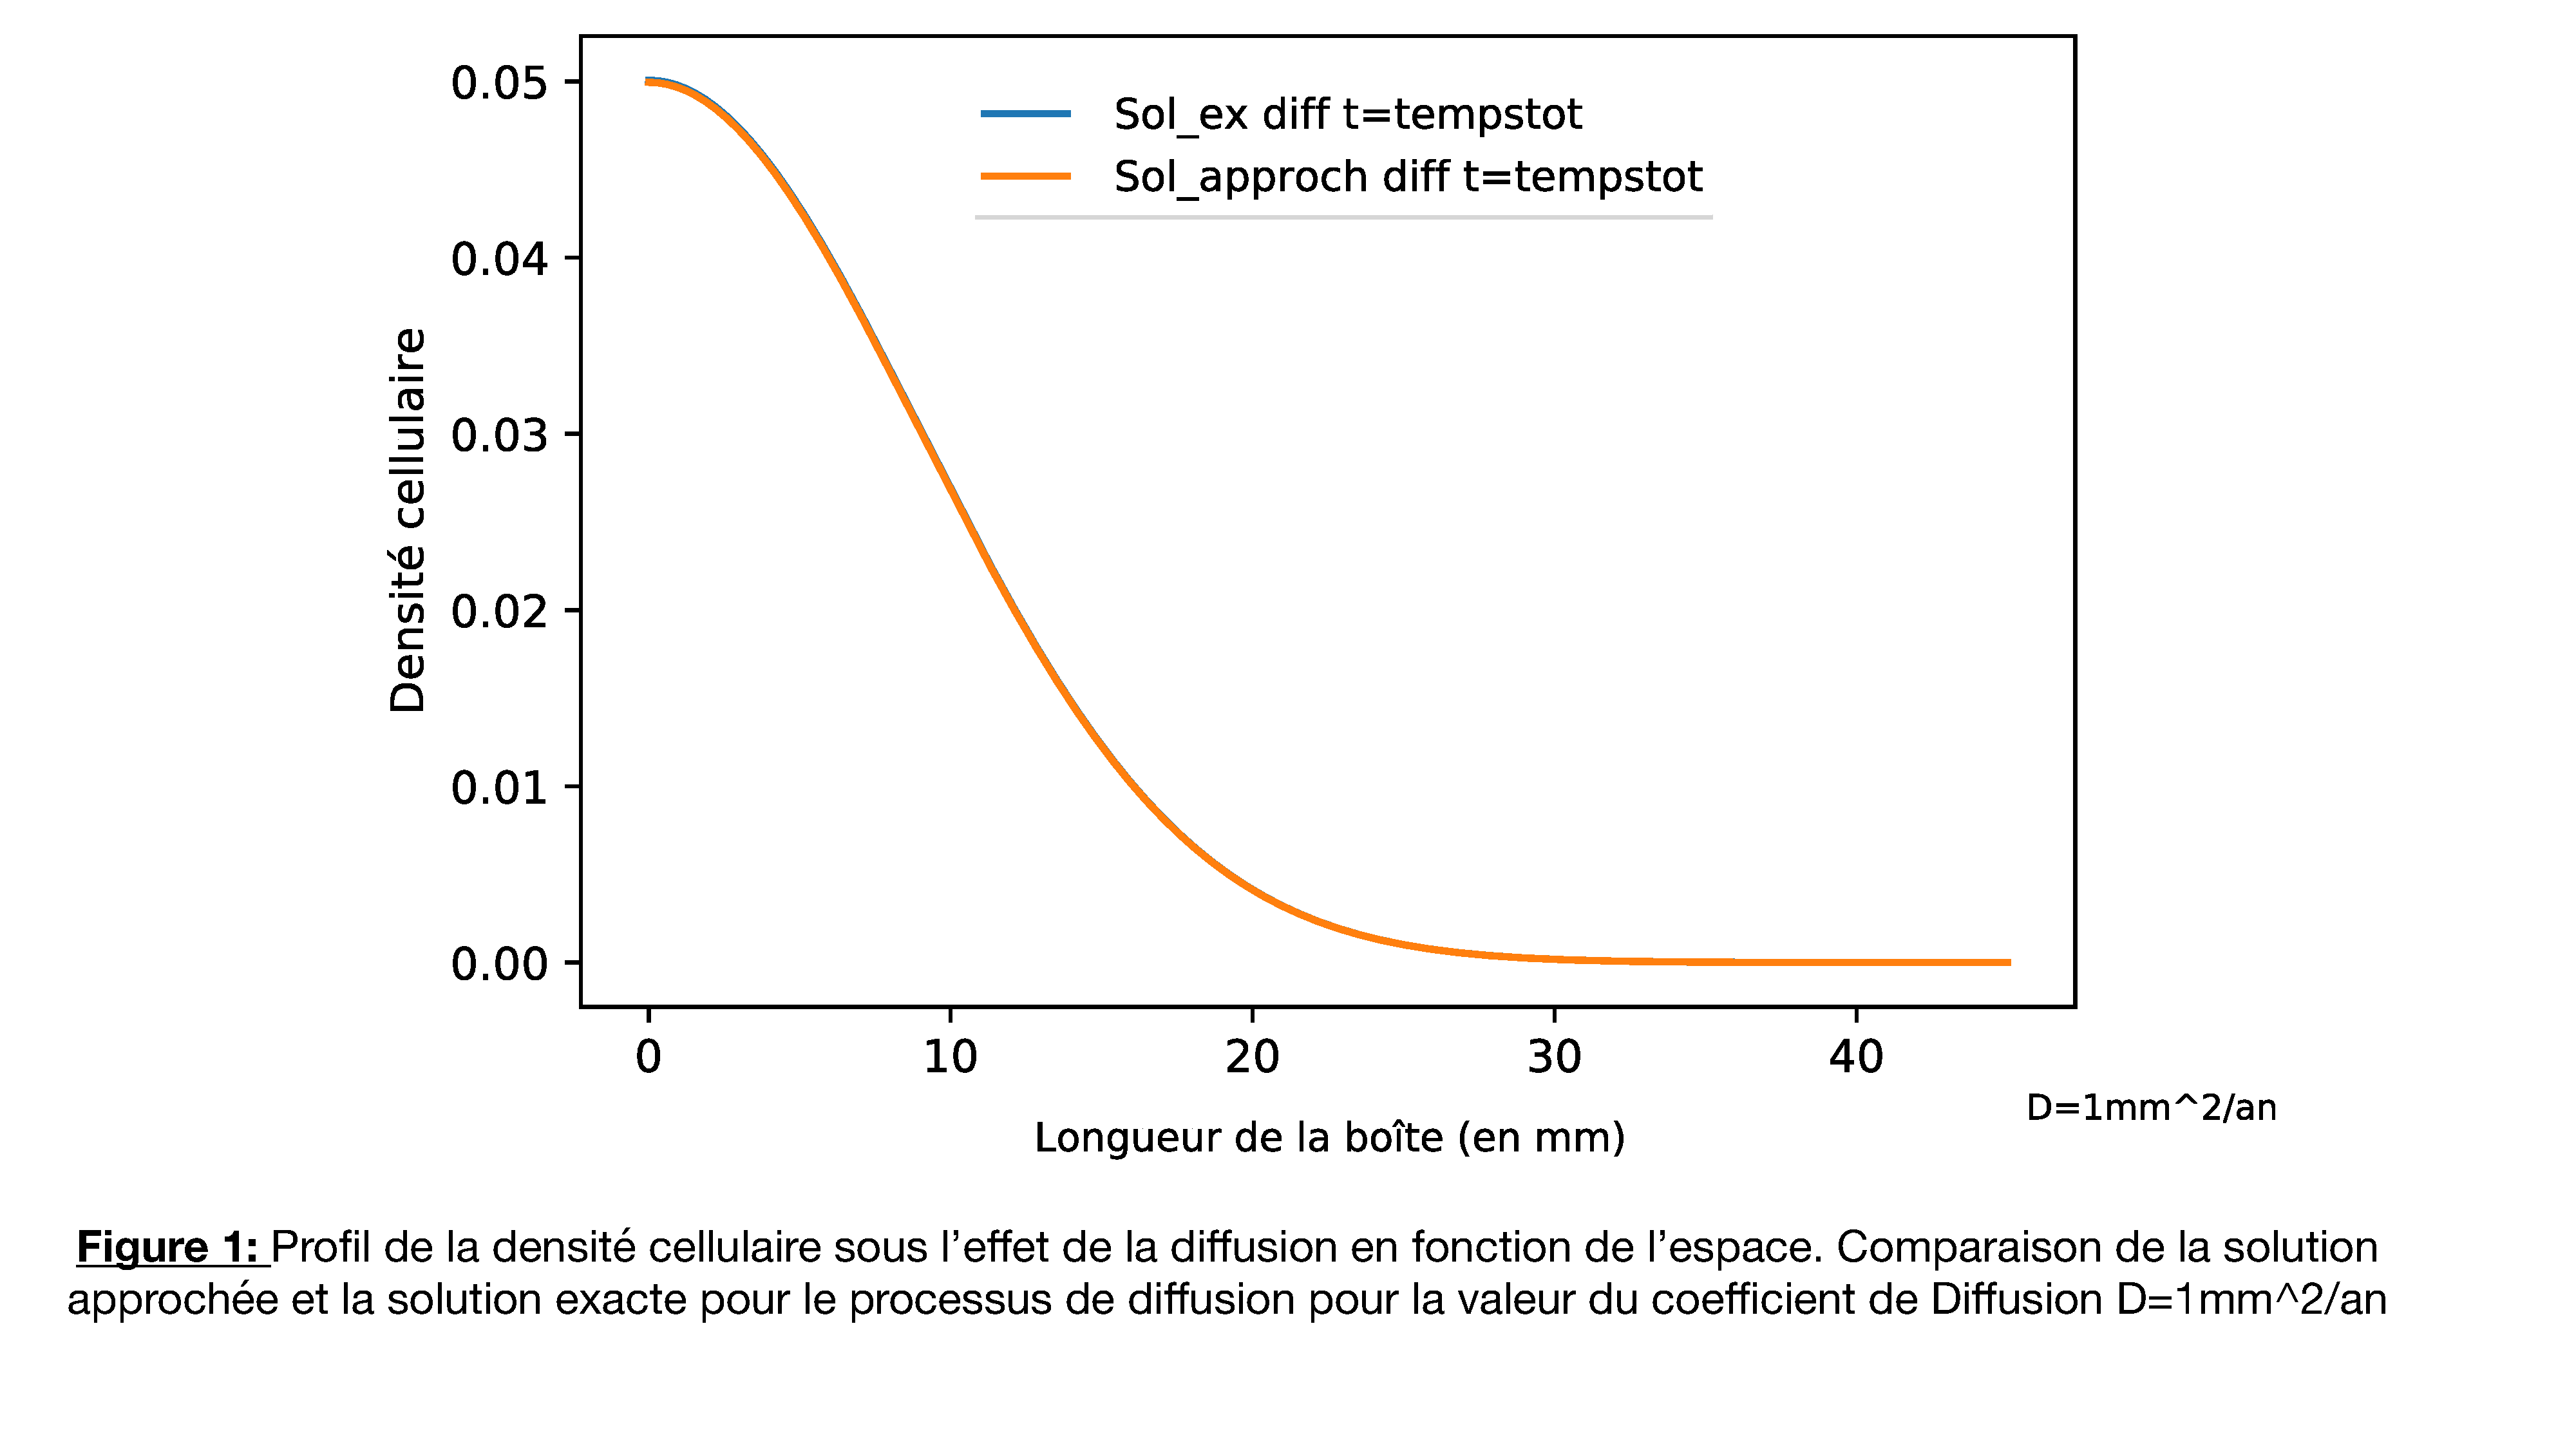
\includegraphics[page=1,scale=0.25]{FIGURES.pdf} 
\\
J'ai représenté l'évolution du processus de diffusion prolifération sans Radiothérapie (voir Figure 2.a p.10). En partant des condition initiales de la marche, on observe une brusque diminution de la densité cellulaire au tout début. Au bout d'un certain temps, on constate que la densité cellulaire commmence à augmenter au centre jusqu'à atteindre la saturation en 1.0. À partir de ce moment, on observe une diffusion et prolifération partant du centre. 
L'allure du rayon est représentée par la Figure suivante (Voir Figure 2.c p.10). On va choisir pour cette description $\kappa$=1$ans^{-1}$. On constate qu'au début, le rayon est nul, puis commence au bout d'un certain temps à croître linéairement.  Afin de mieux pouvoir voir les variations au sein de la courbe du rayon, j'ai représenté l'évolution de la pente (Voir Figure 2.b p.10). En effet, on remarque que la vitesse de croissance du rayon est très importante. Cependant, cette dernière diminue en fonction du temps et plafonne en atteignant une vitesse constante $2\sqrt{D\kappa}$. On a défini la valeur $t_lim$ comme étant le moment au bout duquel le rayon tumoral commence à croître de façon constante. On précisera son calcul en Annexe (Voir Annexe c). 
\\
\\
\includegraphics[page=2,scale=0.25]{FIGURES.pdf} 
\\

\subsubsection{Phase Silencieuse}
On appelle, phase silencieuse, l'intervalle de temps pour lequel le rayon tumoral évolue mais reste en dessous du seuil de détection, et donc, est indétectable {ref. Figure c}. L'étude en profondeur de la solution exacte peut nous permettre de mettre en évidence la relation des paramètres comme $\kappa$ , dans l'évolution de cette phase silencieuse. 
À partir du développement (Voir 2.5.d p.8), on obtient $x^2(t) = (-ln(C^{*}\frac{t_0}{t + t_0})^{1/2} + \kappa t ) 4D(t+t_0)$. 
Donc, pour $\kappa t \leq ln(C^{*}(\frac{t_0 + t}{t_0})^{1/2}$ (resp $\kappa t \geq ln(C^{*}(\frac{t_0 + t}{t_0})^{1/2}$ ), le rayon tumoral est en dessous du seuil de détection (resp. en dessus). On retrouve alors le moment à partir duquel le rayon tumoral devient détectable à partir de l'équation,et par conséquent l'intervalle de la phase silencieuse à partir de la formule dépendante de $\kappa$:
$\kappa t = ln(C^{*}(\frac{t_0 + t}{t_0})^{1/2})$ (Voir Figure 2.c p.10) 
Comme expliqué au point (Voir 2.4.d p.8), la solution exacte utilise des conditions initiales sans terme de saturation (1-C), ce qui n'est pas notre cas. Dans ce dernier, on ne peut espérer qu'un résultat proche à celui de la gaussienne.  
\\
\subsection{Après l'application de la Radiothérapie}
\\
\subsubsection{Profil après une session de Radiothérapie}
L'effet de la Radiothérapie se traduit sous forme d'une forte diminution de la densité cellulaire (Voir Figure 3.a couleur Jaune et Rose p.11), suivie d'une réaugmentation au bout d'un certain temps (Voir Figure 3.a  courbes violette, bleue et verte p.11), conduisant à nouveau à la saturation des tissus (Voir Figure 3.a courbes noires p.11). 
\\
\\
\includegraphics[page=3,scale=0.25]{FIGURES.pdf}
\\
\\
Lors qu'on applique la fonction calculant le rayon de la tumeur sur ce nouveau profil (Voir Figure 3.b p.11), on remarque une diminution du rayon, à l'origine d'un creux, puis une réaugmentation du rayon tumoral au bout d'un certain intervalle de temps.
\\

\subsubsection{Etude des paramètres p et M}
\\
Pour la suite, j'ai décidé d'étudier l'influence des paramètres p et M sur le rayon tumoral après la Radiothérapie. 
Pour cela, on analysera des caractéristiques particulières, notamment, la variation du rayon et de la pente, les intervalles $\Delta G$ (se traduisant par un gain de temps de vie en raison du ralentissement de l'évolution du rayon tumoral) et la valeur du rayon minimal après la Radiothérapie.
\\
\\
En fixant la fraction des cellules atteintes par la Radiothérapie à $p$=0.9, et testant plusieurs valeurs de $M$, on remarque une certaine influence du taux de mort cellulaire sur la valeur du rayon tumoral s'accentuant à mesure qu'on augmente M (Voir Figure 4.a et 4.c p.10). Ceci se traduit par une chute de la pente du rayon tumoral (Voir Figure 4.b p.12). On remarque en parallèlle une influence en second plan du paramètre p sur cette variation du rayon tumoral augmentant le rendement du traitement (Voir Figure 4.c et Annexe d Figure C.b p.16). 
\\
\\
\includegraphics[page=4,scale=0.23]{FIGURES.pdf}
\\
\\
\\
En fixant en parallèle la valeur de $M$ à $2.5$ans$^{-1}$ et testant plusieurs valeurs de $p$, on constate l'influence de $p$ sur la durée de l'intervalle $\Delta G$ (Voir Figure 5.a, 5.b p.12). Ce qui se traduit biologiquement par une durée plus étendue de l'efficacité du traitement. \\
\\
\\
\includegraphics[page=5,scale=0.23]{FIGURES.pdf}
\\
\\
\\
 Au contraire que pour M, on remarque que $\Delta G$ varie en fonction de p (Voir Figure 5.c p.12), alors que les valeurs du rayon minimal ont une allure indentique à valeurs dépendantes de M (Voir Annexe d Figure C.a p.16). 
\\
\newpage
\\
\section{Conclusions et Discussions :}
L'équation de Fisher-Kolmogorov permet de décrire la croissance logistique d'une population se dispersant via diffusion linéaire. La dichotomie suscitée par les procéssus de diffusion et prolifération permet l'adaptation de l'équation er donc la mise en place du modèle de diffusion prolifération. L'équation de ce modèle et sa discrétisation nous a permis d'étudier l'évolution de la tumeur sous deux conditions en particulier, en conditions normales sans application d'aucun traitement, puis, après une session de radiothérapie. 
\\
\\
Dans un premiers temps, la modélisation de l'évolution tumorale sans l'application de la Radiothérapie nous a permis de distinguer deux paramètres jouant un rôle majeur dans l'évolution du rayon tumoral, D (en $mm^2/an$ et $\kappa$ (en $ an^{-1} $). En effet, le coefficient D permet de déterminer le caractère diffusif de la tumeur. En parallèlle, $\kappa$ a un rôle bien défini dans la durée de la phase silencieuse. On a pu remarqué que plus $\kappa$ devient grand (resp. petit), plus la capacité proliférative des cellules augmente, et donc, plus rayon tumoral se développe rapidement (resp. lentement). Donc, plus la durée de la phase silencieuse est réduite (resp. prolongée). Les études précedents de ces paramètres nous a permis de fixer pour la suite $\kappa$ = 1 an$^{-1}$ et $D$ = 1 $mm^2/an $.
\\
\\
La comparaison entre nos deux conditions nous a permis de comprendre l'effet de la RT sur la tumeur. Le mode d'action de la RT nous a permis de définir deux population distinctes intéragissant entre elles et dont leur somme au moment défini la population totale. On distingue d'une part les cellules tumorales non atteintes par la radiothérapie $C_n$, puis d'autre part les cellules atteintes par la radiothérapie $C_d$.  C'est ici où l'on comprend l'influence du paramètre p pour l'étude de la Radiothérapie. En effet, ce dernier nous permettra de déterminer la proportion de cellules atteintes par la RT, et donc de définir les population $C_n$ et $C_d$. La population $C_d$ regroupe deux sous-populations, les cellules avec des lessions au niveau d'une simple hélice de la chaîne d'ADN, réparable et donc regroupant les cellules allant survivre, puis les cellules avec des lessions au niveau de la double chaîne d'ADN, non réparables et conduisant à l'apoptose cellulaire. On comprend ici le rôle du paramètre $M$ (en ans$^{-1}$), permettant de définir l'ensemble des cellules allant être conduites à l'apoptose, ou dont les lésions seront réparés. L'étude de ces deux paramètre va nous permettre d'étudier plusieurs caractéristiques intéréssant les médecins, l'intervalle de temps au bout duquel le rayon tumoral retourne à sa valeur initiale, $\Delta G$ et la valeur minimale du rayon. Nos résultats nous ont permis de mettre en évidence le rôle de p dans l'intervalle $\Delta$G. On pourrait expliquer cela par le faite que, plus la proportion de cellules atteintes par la RT est élevée, plus la population $C_d$ sera réduite, et plus de temps sera nécéssaire pour atteindre à nouveau le rayon initial. Autrement dit, plus le traitement serà efficace pendant longtemps. De même, on a remarqué l'influence de M dans la valeur du rayon minimal. Ainsi, plus la proportion de cellules tumorales atteintes par la RT allant mourir augmente, plus la population totale de cellules va être réduite, et donc on aura un rayon tumoral petit. On peut éventuellement remarquer une légère co-influence entre $p$ et $M$ ce traduisant par une efficacité du traitement plus accrue pour des grandes valeurs de $p$ et $M$ (Voir Annexe d Figure C.b p.16 et Figure 4.c p.12 )  c'est à dire, lorsque la RT atteint non seulement une grande proportion de la population, mais aussi, lorsqu'une grande partie de ces dernières est conduite en apoptose. 
\\
\\
Ceci étant dit, le prochain pas concernerait l'adaptation du modèle en conditons 3-D. Malheuresement, la courte durée du stage m'oblige à finir mes recherches pour l'instant. J'aurais bien aimé adapter mon modèle en 3 dimensions et avoir eu l'occasion de voir mes résultats plus tangiblement. D'autre part, j'aurais également aimé travailler sur la comparaison du modèle aux bases de données des patients. J'ai beaucoup profité ce stage, ce dernier m'a permis de retrouver une direction dans laquelle orienter ma carrière proféssionnelle. Je me permet ainsi d'affirmer que, ceci n'est pas un point final, mais plutôt un point virgule. 
\\



\section{Bibliographie :}

\bibliographystyle{unsrt}
\bibliography{bibliob.bib}
	


\vspace{13cm}
\def\theequation{\Roman{equation}}
\section{Annexe}
\\
\\
\subsubsection{Modes d'action et effets de la radiation}
\\
Cette Figure apparrtient à la page 196 de l'article \cite{h} .
\\
\includegraphics[page=6,scale=0.26]{FIGURES.pdf}
\\
\subsubsection{Figures de la Diffusion et de la prolifération}
\\
\includegraphics[page=7,scale=0.25]{FIGURES.pdf}
\\
\subsubsection{Calcul du $t_{lim}$}
\\
Le t0 représente le moment à partir duquel, la vitesse de front devient constante à $2\sqrt{D\kappa}$ et donc, le rayon de la tumeur croit de façon constante. 
Pour déterminer le $t_{lim}$, on appliquera à chaque temps fixé, une fonction qui réenverra l'indice du premier terme égal à $2\sqrt{D\kappa}$. Plus particulièerement, on analysera le moment où la valeur $2\sqrt{D\kappa}$ est ntre deux indices consécutifs, puis on assignera le point milieu des deux indices fois dt, comme le $t_{lim}$. 
\\
\subsubsection{Influence en second plan des paramètres p et M}
\\
\includegraphics[page=8,scale=0.25]{FIGURES.pdf}

\subsubsection{Lien vers les scripts}
\\
Faire click \href{run:Stage 2021/suite rapport/CodesPython.tex}{\textbf{ici}} pour ouvrir le pdf contenant les codes Python.

\end{document}

